% !TeX spellcheck = ru_RU
% В этом файле следует писать текст работы, разбивая его на
% разделы (section), подразделы (subsection) и, если нужно,
% главы (chapter).

% Предварительно следует указать необходимую информацию
% в файле SETUP.tex

%% В этот файл не предполагается вносить изменения

% В этом файле следует указать информацию о себе
% и выполняемой работе.

\documentclass [fontsize=14pt, paper=a4, pagesize, DIV=calc]%
{scrreprt}
% ВНИМАНИЕ! Для использования глав поменять
% scrartcl на scrreprt

% Здесь ничего не менять
\usepackage [T2A] {fontenc}   % Кириллица в PDF файле
\usepackage [utf8] {inputenc} % Кодировка текста: utf-8
\usepackage [russian] {babel} % Переносы, лигатуры

\usepackage[dvipsnames]{xcolor}
\usepackage{listings}

\usepackage{amsmath} % column vector, matrix
\usepackage{svg}

\usepackage{caption}
\usepackage{subcaption}
\usepackage{csquotes} % big quotations

%%%%%%%%%%%%%%%%%%%%%%%%%%%%%%%%%%%%%%%%%%%%%%%%%%%%%%%%%%%%%%%%%%%%%%%%
% Создание макроса управления элементами, специфичными
% для вида работы (курс., бак., маг.)
% Здесь ничего не менять:
\usepackage{ifthen}
\newcounter{worktype}
\newcommand{\typeOfWork}[1]
{
	\setcounter{worktype}{#1}
}

% ВНИМАНИЕ!
% Укажите тип работы: 0 - курсовая, 1 - бак., 2 - маг.,
% 3 - бакалаврская с главами.
\typeOfWork{2}
% Считается, что курсовая и бак. бьются на разделы (section) и
% подразделы (subsection), а маг. — на главы (chapter), разделы и
%  подразделы. Если хочется,
% чтобы бак. была с главами (например, если она большая),
% надо выбрать опцию 3.

% Если при выборе 2 или 3 вы забудете поменять класс
% документа на scrreprt (см. выше, в самом начале),
% то получите ошибку:
% ./aux/appearance.tex:52: Package scrbase Error: unknown option ` chapterprefix=

%%%%%%%%%%%%%%%%%%%%%%%%%%%%%%%%%%%%%%%%%%%%%%%%%%%%%%%%%%%%%%%%%%%%%%%%
% Информация об авторе и работе для титульной страницы

\usepackage {titling}

% Имя автора #ИСПРАВИТЬ!
\newcommand {\byme}{%
	\textbf{Каспаров~Александр~Валерьевич}%
}

% Научный руководитель #ИСПРАВИТЬ!
\newcommand{\supervisor}%
{к.ф-м.н. Оганесян Павел Артурович}

% Рецензент #ИСПРАВИТЬ!
\newcommand{\reviewer}%
{к.ф-м.н. Колесников Алексей Михайлович}


% Год публикации
\date{2022}

% Название работы #ИСПРАВИТЬ!
\title{\textbf{Разработка мобильного приложения для геймифицированных тренировок на основе геоданных}}

% Кафедра
%

\newcommand {\direction} {%
	02.\ifthenelse{\value{worktype} = 2}{04}{03}.02 --- Фундаментальная информатика и информационные технологии%
}

% Заведующий кафедрой #ИСПРАВИТЬ!
\newcommand{\headOfDepartment}{Угольницкий Г.\,А.}

% Направленность магистерской программы #ИСПРАВИТЬ!
\newcommand{\programme}{``Разработка мобильных приложений и компьютерных игр''}

% Руководитель магистерской программы #ИСПРАВИТЬ!
\newcommand{\headOfProgramme}{к.т.н. Демяненко Я.\,М.}

% Кафедра #ИСПРАВИТЬ!
\newcommand{\department}{Кафедра прикладной математики и программирования}

%%%%%%%%%%%%%%%%%%%%%%%%%%%%%%%%%%%%%%%%%%%%%%%%%%%%%%%%%%%%%%%%%%%%%%%%
% Другие настраиваемые элементы текста

% Листинги с исходным кодом программ: укажите язык программирования
\usepackage{listings}
\lstset{
	language=[ISO]C++,%  Язык указать здесь
	basicstyle=\small\ttfamily,
	breaklines=true,%
	showstringspaces=false%
	inputencoding=utf8x%
}
% полный список языков, поддерживаемых данным пакетом, есть,
% например, здесь (стр. 13):
% ftp://ftp.tex.ac.uk/tex-archive/macros/latex/contrib/listings/listings.pdf

% Нумерация списков: можно при необходимести
% изменять вид нумерации (например, добавлять правую скобку).
% По умолчанию буду списки вида:
% 1.
% 2.
% Изменять вид нумерации можно в начале нумерации:
% \begin{enumerate}[1)] (В квадратных скобках указан желаемый вид)
\usepackage[shortlabels]{enumitem}
\setlist[enumerate, 1]{1.}

% Гиперссылки: настройте внешний вид ссылок
\usepackage%
[pdftex,unicode,pdfborder={0 0 0},draft=false,%backref=page,
hidelinks, % убрать, если хочется видеть ссылки: это
% удобно в PDF файле, но не должно появиться на печати
bookmarks=true,bookmarksnumbered=false,bookmarksopen=false]%
{hyperref}


\usepackage {amsmath}      % Больше математики
\usepackage {amssymb}
\usepackage {textcase}     % Преобразование к верхнему регистру
\usepackage {indentfirst}  % Красная строка первого абзаца в разделе
\usepackage {pdfpages}     % Inject PDF files
\usepackage {easyReview}
\usepackage {pgf-pie}
\usepackage {etoolbox}
\usepackage {verbatim}


\usepackage {fancyvrb}     % Листинги: определяем своё окружение Verb
\DefineVerbatimEnvironment% с уменьшенным шрифтом
	{Verb}{Verbatim}
	{fontsize=\small}


% Вставка рисунков
\usepackage {graphicx}

% Общее оформление
% ----------------------------------------------------------------
% Настройка внешнего вида

%%% Шрифты

% если закомментировать всё — консервативная гарнитура Computer Modern
\usepackage{paratype} % профессиональные свободные шрифты
%\usepackage {droid}  % неплохие свободные шрифты от Google
%\usepackage{mathptmx}
%\usepackage {mmasym}
%\usepackage {psfonts}
%\usepackage{lmodern}
%var1: lh additions for bold concrete fonts
%\usepackage{lh-t2axccr}
%var2: the package below could be covered with fd-files
%\usepackage{lh-t2accr}
%\usepackage {pscyr}
\usepackage{tabularx}

% Геометрия текста

\usepackage{setspace}       % Межстрочный интервал
\onehalfspacing

\newlength\MyIndent
\setlength\MyIndent{1.25cm} %1.25
\setlength{\parindent}{\MyIndent} % Абзацный отступ
\frenchspacing            % Отключение лишних отступов после точек
\KOMAoptions{%
    DIV=calc,         % Пересчёт геометрии
    numbers=endperiod % точки после номеров разделов
}

                          %   Консервативный вариант:
\usepackage                % ручное задание геометрии
[%                         % (не рекомендуется в проф. типографии)
  left=3cm,
  right=1.5cm,
  top=2cm,
  bottom=2cm,
  includefoot,
  footskip = 1cm
] %
  {geometry}

%%% Заголовки

\ifthenelse{\equal{\theworktype}{2}}{%
\KOMAoptions{%
    numbers=endperiod,% точки после номеров разделов
    headings=normal,   % размеры заголовков поменьше стандартных
    chapterprefix=true,% Печатать слово Глава в магистерской
    appendixprefix=true% Печатать слово Приложение
}
}
{% Печатать слово Приложение даже если нет глав
\newcommand*{\appendixmore}{%
	\renewcommand*{\sectionformat}{%
		\appendixname~\thesection\autodot\enskip}
	\renewcommand*{\sectionmarkformat}{%
		\appendixname~\thesection\autodot\enskip}
}
}

% шрифт для оформления глав и названия содержания
\newcommand{\SuperFont}{\Large\sffamily\bfseries}

% Заголовок главы
\ifthenelse{\value{worktype} > 1}{%
\renewcommand{\SuperFont}{\Large\normalfont\sffamily}
\newcommand{\CentSuperFont}{\centering\SuperFont}
\usepackage{fncychap}
\ChNameVar{\SuperFont}
\ChNumVar{\CentSuperFont}
\ChTitleVar{\CentSuperFont}
\ChNameUpperCase
\ChTitleUpperCase
}

% Заголовок (под)раздела с абзацного отступа
\addtokomafont{sectioning}{\hspace{\MyIndent}}

\renewcommand*{\captionformat}{~---~}
\renewcommand*{\figureformat}{Рисунок~\thefigure}

% Плавающие листинги
\usepackage{float}
\floatstyle{ruled}
\floatname{ListingEnv}{Листинг}
\newfloat{ListingEnv}{htbp}{lol}[section]

% точка после номера листинга
\makeatletter
\renewcommand\floatc@ruled[2]{{\@fs@cfont #1.} #2\par}
\makeatother


%%% Оглавление
\usepackage{tocloft}

% шрифт и положение заголовка
\ifthenelse{\value{worktype} > 1}{%
\renewcommand{\cfttoctitlefont}{\hfil\SuperFont\MakeUppercase}
}{
\renewcommand{\cfttoctitlefont}{\hfil\SuperFont}
}

% слово Глава
\usepackage{calc}
\ifthenelse{\value{worktype} > 1}{%
\renewcommand{\cftchappresnum}{Глава }
\addtolength{\cftchapnumwidth}{\widthof{Глава }}
}

% Очищаем оформление названий старших элементов в оглавлении
\ifthenelse{\value{worktype} > 1}{%
\renewcommand{\cftchapfont}{}
\renewcommand{\cftchappagefont}{}
}{
\renewcommand{\cftsecfont}{}
\renewcommand{\cftsecpagefont}{}
}

% Точки после верхних элементов оглавления
\renewcommand{\cftsecdotsep}{\cftdotsep}
%\newcommand{\cftchapdotsep}{\cftdotsep}

\ifthenelse{\value{worktype} > 1}{%
    \renewcommand{\cftchapaftersnum}{.}
}{}
\renewcommand{\cftsecaftersnum}{.}
\renewcommand{\cftsubsecaftersnum}{.}
\renewcommand{\cftsubsubsecaftersnum}{.}

%%% Списки (enumitem)

\usepackage {enumitem}      % Списки с настройкой отступов
\setlist %
{ %
  leftmargin = \parindent, itemsep=.5ex, topsep=.4ex
} %

% По ГОСТу нумерация должны быть буквами: а, б...
%\makeatletter
%    \AddEnumerateCounter{\asbuk}{\@asbuk}{м)}
%\makeatother
%\renewcommand{\labelenumi}{\asbuk{enumi})}
%\renewcommand{\labelenumii}{\arabic{enumii})}

%%% Таблицы: выбрать более подходящие

\usepackage{booktabs} % считаются наиболее профессионально выполненными
%\usepackage{ltablex}
%\newcolumntype {L} {>{---}l}

%%% Библиография

\usepackage{csquotes}        % Оформление списка литературы
\usepackage[
  backend=biber,
  hyperref=auto,
  sorting=none, % сортировка в порядке встречаемости ссылок
  language=auto,
  citestyle=gost-numeric,
  bibstyle=gost-numeric
]{biblatex}
\addbibresource{biblio.bib} % Файл с лит.источниками

% Настройка величины отступа в списке
\ifthenelse{\value{worktype} < 2}{%
\defbibenvironment{bibliography}
  {\list
     {\printtext[labelnumberwidth]{%
    \printfield{prefixnumber}%
    \printfield{labelnumber}}}
     {\setlength{\labelwidth}{\labelnumberwidth}%
      \setlength{\leftmargin}{\labelwidth}%
      \setlength{\labelsep}{\dimexpr\MyIndent-\labelwidth\relax}% <----- default is \biblabelsep
      \addtolength{\leftmargin}{\labelsep}%
      \setlength{\itemsep}{\bibitemsep}%
      \setlength{\parsep}{\bibparsep}}%
      \renewcommand*{\makelabel}[1]{\hss##1}}
  {\endlist}
  {\item}
}{}

% ----------------------------------------------------------------
% Настройка переносов и разрывов страниц

\binoppenalty = 10000      % Запрет переносов строк в формулах
\relpenalty = 10000        %

\sloppy                    % Не выходить за границы бокса
%\tolerance = 400          % или более точно
\clubpenalty = 10000       % Запрет разрывов страниц после первой
\widowpenalty = 10000      % и перед предпоследней строкой абзаца

% ----------------------------

\lstdefinelanguage{Kotlin}{
	comment=[l]{//},
	commentstyle={\color{gray}\ttfamily},
	emph={filter, first, firstOrNull, forEach, lazy, map, mapNotNull, println},
	emphstyle={\color{OrangeRed}},
	identifierstyle=\color{black},
	keywords={!in, !is, abstract, actual, annotation, as, as?, break, by, catch, class, companion, const, constructor, continue, crossinline, data, delegate, do, dynamic, else, enum, expect, external, false, field, file, final, finally, for, fun, get, if, import, in, infix, init, inline, inner, interface, internal, is, lateinit, noinline, null, object, open, operator, out, override, package, param, private, property, protected, public, receiveris, reified, return, return@, sealed, set, setparam, super, suspend, tailrec, this, throw, true, try, typealias, typeof, val, var, vararg, when, where, while},
	keywordstyle={\color{NavyBlue}\bfseries},
	morecomment=[s]{/*}{*/},
	morestring=[b]",
	morestring=[s]{"""*}{*"""},
	ndkeywords={@Test, @Deprecated, @JvmField, @JvmName, @JvmOverloads, @JvmStatic, @JvmSynthetic, Array, Byte, Double, Float, Int, Integer, Iterable, Long, Runnable, Short, String, Any, Unit, Nothing},
	ndkeywordstyle={\color{BurntOrange}\bfseries},
	sensitive=true,
	stringstyle={\color{ForestGreen}\ttfamily},
}

% Стили для окружений типа Определение, Теорема...
% Оформление теорем (ntheorem)

\usepackage [thmmarks, amsmath] {ntheorem}
\theorempreskipamount 0.6cm

\theoremstyle {plain} %
\theoremheaderfont {\normalfont \bfseries} %
\theorembodyfont {\slshape} %
\theoremsymbol {\ensuremath {_\Box}} %
\theoremseparator {:} %
\newtheorem {mystatement} {Утверждение} [section] %
\newtheorem {mylemma} {Лемма} [section] %
\newtheorem {mycorollary} {Следствие} [section] %

\theoremstyle {nonumberplain} %
\theoremseparator {.} %
\theoremsymbol {\ensuremath {_\diamondsuit}} %
\newtheorem {mydefinition} {Определение} %

\theoremstyle {plain} %
\theoremheaderfont {\normalfont \bfseries} 
\theorembodyfont {\normalfont} 
%\theoremsymbol {\ensuremath {_\Box}} %
\theoremseparator {.} %
\newtheorem {mytask} {Задача} [section]%
\renewcommand{\themytask}{\arabic{mytask}}

\theoremheaderfont {\scshape} %
\theorembodyfont {\upshape} %
\theoremstyle {nonumberplain} %
\theoremseparator {} %
\theoremsymbol {\rule {1ex} {1ex}} %
\newtheorem {myproof} {Доказательство} %

\theorembodyfont {\upshape} %
%\theoremindent 0.5cm
\theoremstyle {nonumberbreak} \theoremseparator {\\} %
\theoremsymbol {\ensuremath {\ast}} %
\newtheorem {myexample} {Пример} %
\newtheorem {myexamples} {Примеры} %

\theoremheaderfont {\itshape} %
\theorembodyfont {\upshape} %
\theoremstyle {nonumberplain} %
\theoremseparator {:} %
\theoremsymbol {\ensuremath {_\triangle}} %
\newtheorem {myremark} {Замечание} %
\theoremstyle {nonumberbreak} %
\newtheorem {myremarks} {Замечания} %


% Титульный лист
% Макросы настройки титульной страницы
% В этот файл не предполагается вносить изменения

%\usepackage {showframe}

% Вертикальные отступы на титульной странице
\newcommand{\vgap}{\vspace{16pt}}

% Помещение города и даты в нижний колонтитул
\usepackage{scrlayer}
\DeclareNewLayer[
foot,
foreground,
contents={%
	\raisebox{\dp\strutbox}[\layerheight][0pt]{%
		\parbox[b]{\layerwidth}{\centering Ростов-на-Дону -- \thedate%
			\\\mbox{}
	}}%
}
]{titlepage.foot.fg}
\DeclareNewPageStyleByLayers{titlepage}{titlepage.foot.fg}


\AtBeginDocument %
{ %
	%
	\begin{titlepage}
		%
		\thispagestyle{titlepage}
		
		{\centering
			%
			\MakeTextUppercase {МИНОБРНАУКИ РОССИИ}
			
			\vgap
			
			Федеральное государственное автономное образовательное\\
			учреждение высшего образования\\
			\textquote{Южный федеральный университет}
			
			\vgap
			
			Институт математики, механики \\ и компьютерных наук
			имени~И.\,И.\,Воровича
			
			\vgap
			
			\ifthenelse{\value{worktype} = 1 \OR \value{worktype} = 3}{
				\department
			}{}
			
			
			\vgap
			\vgap
			
			\byme
			
			\vgap
			\vgap
			
			\MakeTextUppercase{\thetitle}
			
			\vgap
			\vgap
			
			\MakeTextUppercase{Выпускная квалификационная работа} \\ 
			по направлению подготовки \\
			\direction
			\ifthenelse{\value{worktype} = 2}{
				\\ направленность программы \\
				 \programme \\
			}{}
			
			\vgap
			\vgap
			
			\textbf{Научный руководитель} -- \\
			\supervisor
			\ifthenelse{\value{worktype} = 2}{
				\\ \textbf{Рецензент} -- \\
				\reviewer
			}{}
			
			\vspace {\fill}
			
			\ifthenelse{\value{worktype} = 1 \OR \value{worktype} = 3}{
				
				\begin{flushleft}
					Допущено к защите:\\
					заведующий кафедрой \underline{\hspace{6.8cm}}\headOfDepartment
				\end{flushleft}
			}{}
		
			\ifthenelse{\value{worktype} = 2}{
				
				\begin{flushleft}
					Допущено к защите:\\
					руководитель\\
					образовательной программы \underline{\hspace{4cm}}\headOfProgramme
				\end{flushleft}
			}{}
			
			
			\vspace {\fill}
			%Ростов-на-Дону
			
			%\thedate
			
	}\end{titlepage}
	%
	%
	\tableofcontents
	%
	\clearpage
} %


% Команды для использования в тексте работы

% макросы для начала введения и заключения
\newcommand{\Task}{\addsec{Постановка задачи}}
\ifthenelse{\value{worktype} > 1}{%
	\renewcommand{\Task}{\addchap{Постановка задачи}}%
}

% макросы для начала введения и заключения
\newcommand{\Intro}{\addsec{Введение}}
\ifthenelse{\value{worktype} > 1}{%
    \renewcommand{\Intro}{\addchap{Введение}}%
}

\newcommand{\Conc}{\addsec{Заключение}}
\ifthenelse{\value{worktype} > 1}{%
    \renewcommand{\Conc}{\addchap{Заключение}}%
}

% Правильные значки для нестрогих неравенств и пустого множества
\renewcommand {\le} {\leqslant}
\renewcommand {\ge} {\geqslant}
\renewcommand {\emptyset} {\varnothing}

% N ажурное: натуральные числа
\newcommand {\N} {\ensuremath{\mathbb N}}

% значок С++ — используйте команду \cpp
\newcommand{\cpp}{%
C\nolinebreak\hspace{-.05em}%
\raisebox{.2ex}{+}\nolinebreak\hspace{-.10em}%
\raisebox{.2ex}{+}%
}

% Неразрывный дефис, который допускает перенос внутри слов,
% типа жёлто-синий: нужно писать жёлто"/синий.
\makeatletter
    \defineshorthand[russian]{"/}{\mbox{-}\bbl@allowhyphens}
\makeatother


\endinput

% Конец файла


\begin{document}

\Intro

Геймификация спорта сегодня особенно актуальна~\autocite{gamification}: после введения ограничений в связи с распространением COVID-19 активность людей по всему миру начала неуклонно снижаться. В этот момент стали популярны самостоятельные тренировки в стиле ``несколько кругов по квартире'' или ``по лестнице подъезда туда-обратно''. Потребность в спорте остаётся актуальна и сейчас, когда ограничения постепенно снимаются. При этом, со временем, у многих людей, не привыкших к спорту, но чувствующих его необходимость в своей жизни, снижается уровень мотивации к занятиям разного рода активностями. 

Игра, будучи одной из форм деятельности человека, по определению является свободной развивающей деятельностью, выполняемой субъектом по желанию и ради удовольствия от процесса. Считается, что у такой формы деятельности есть четкий набор правил, а сама игра должна подготовить ребенка ко взрослой деятельности.

Однако в современном мире все меняется, и игра постепенно выходит на один уровень с остальными базовыми формами деятельности человека. При этом такая игра не готовит ко взрослым активностям, а представляет из себя комплиментарную сущность, которая добавляет то самое удовольствие от процесса, во время занятий другой формой деятельности. Такой подход к добавлению игровых элементов в некоторую деятельность, направленный на обучение деятельности или получение от неё большего удовлетворения как от процесса, принято называть геймификацией.  

Многие эксперты считают, что в современную эпоху упрощения и автоматизации геймификацию имеет смысл применять во всех сферах человеческой жизни, от медицины и до маркетинга.

Некоторое время назад, в рамках курса по гейм-дизайну в магистратуре ИММиКН, была рождена идея приложения, которое могло бы геймифицировать процесс беговых тренировок. После написания серьезного дизайнерского документа и концепции было принято решение воплотить эту идею в жизнь.

Так, данная работа посвящена разработке мобильной игры для геймификации бега с использованием средств геолокации на ОС Android. Приложение получило название ``Run, Listen, Run!''.

Отличительная особенность этого продукта заключается в том, что он позволяет геймифицировать уже имеющиеся у пользователя маршруты для бега, реагировать на состояние пульса и мотивировать к системности тренировок.

Далее в этой работе рассмотрим основную функциональность, методы геймификации бега и некоторые архитектурные решения, примененные нами в приложении ``Run, Listen, Run!''.


 

\newpage

\chapter{Постановка задачи}
В рамках данной работы необходимо разработать схему геймификации занятий бегом, спроектировать архитектуру мобильного приложения для платформы Android, реализовать работу с сервисами геоданных, определить формат данных и представить обработку интерактивных сценариев в этом формате, а так же провести тестирование разработанного приложения.

Под геймификацией~\autocite{gamification} здесь и далее будем понимать внедрение игровых форм взаимодействия в неигровой контекст: работу, учебу и повседневную жизнь.

Разработка данного приложения полностью покрывает требования к компетенциям, получаемым в рамках текущего направления подготовки: элементы геймификации покрывают собой игровую часть, тогда как само приложение в целом является мобильным и соответствует части разработки мобильных приложений.

В рамках постановки задачи по разработке приложения была проведена некоторая подготовительная работа, включающая в себя следующие пункты:
\begin{itemize}
	\item Определение технического стека разработки.
	\item Рассмотрение возможных технических рисков.
	\item Определение базовой функциональности приложения.
	\item Определение методов геймификации.
\end{itemize}
\smallskip
Относительно технического стека разработки было принято решение создавать мобильное приложение под платформу Android. Подробнее об этом расписано в главе \autoref{chap:stack}.


Каждый из возможных технических рисков рисков является отдельным пунктом в списке базовой функциональности игры. Блок функциональности был назван «риском» потому, что при его реализации могут возникнуть непредвиденные трудности, влекущие за собой разного рода риски.

Ниже представлены базовые блоки функциональности:
\begin{enumerate}
	\item Обработка геолокации.
	\item Управление воспроизведением аудио.
	\item Движение игрока по сюжетной линии.
	\item Ядро управления геймификацией активности.
	\item Базовый пользовательский интерфейс.
	\item Отслеживание и ограничение длительности игровой сессии.
\end{enumerate}
\smallskip
Схема геймификации должна включать в себя следующее:
\begin{itemize}
	\item Интерактивный сценарий активности
	\item Безусловная мотивация во время активности
	\item Создание персональных условий соревновательности с системой
	\item Позитивная мотивация по достижении заданных условий
\end{itemize} 
\chapter{Геймификация в играх}
Прежде чем говорить о самой теме, об использовании геолокации в Android, имеет смысл рассказать о жанре игры, которая разработана в рамках данной работы.

Как и в случае с большинством игр, занятия физической активностью в игровой форме вызывают привыкание: пользователи с радостью возвращаются к ним, чтобы справиться со следующим вызовом.
Ключевая особенность приложений, геймифицирующих занятия физической активностью, заключается в том, что для таких занятий как правило не требуется специальное место и время.

\begin{figure}[H]
	\centering
	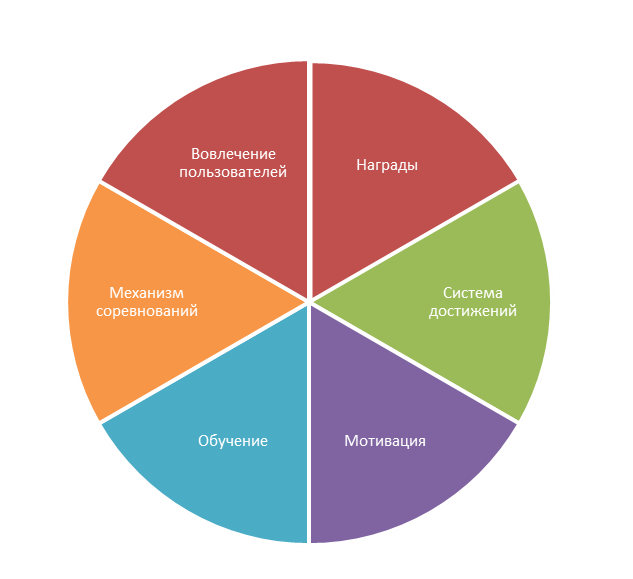
\includegraphics{flesh/gamification/gamification_pie.png}
	\caption{\label{fig:gamification_pie}Схема компонентов геймификации}
\end{figure}

Объединив приложение для тренировок с элементами игрового взаимодействия, можно ввести термин фитнес-игры. 

Фитнес-игра \textendash\space большой жанр игр, преимущественно для мобильных устройств, способствующих поддержанию здоровья игрока. Этот жанр позволяет игрокам геймифицировать свои тренировки: сделать процесс интереснее, веселее, увеличить мотивацию игрока к сохранению стабильной периодичности занятий.

Некоторые игры рассчитаны на одну конкретную активность, другие \textendash\space позволяют комбинировать разные их виды, тогда как третьи\,\textendash\space предлагают свои собственные виды активности для игрока.


Часто такого рода игры обладают минимально достаточным пользовательским интерфейсом:
\begin{itemize}
	\item Информация об активностях
	\item Интерфейс активной игровой сессии
	\item Окно статистики
\end{itemize}

Обычно игры этого жанра тесно интегрируются с устройствами отслеживания состояния игрока, включая, но не ограничиваясь данными с датчиков умных устройств:
\begin{itemize}
	\item Браслеты
	\item Часы
	\item Весы
	\item Смартфоны
	\item Наушники
	\item Умная обувь
\end{itemize}


В качестве примеров можно привести несколько известных игр такого жанра: 
\begin{description}
	\item[Zombies, Run! (2012)] Игра с глубоким погружением, геймифицирующая несколько видов бега и интервальных кардио тренировок. Сюжет разворачивается вокруг небольшого городка, являющегося большой базой выживших при зомби-апокалипсисе. Игрок бежит по открытой территории, собирает предметы в инвентарь, иногда убегает от зомби. Игра содержит несколько сезонов, представляющих из себя продолжения один другого и состоящих из миссий, каждая длинной от 30 до 60 минут.
	\item[Ingress (2013)] Многопользовательская игра с дополненной реальностью. Игра в стиле захвата флага, игроки поделены на две фракции. Потенциально геймифицирует пешие прогулки, не содержит сюжета, при этом позволяет игрокам ``захватывать порталы'' в реальном мире. Основная концепция \textendash\space возможность использовать ``таинственную энергию'' для связи порталов между собой, таким образом покрывая реальную карту многоугольниками с полем одной из двух фракций.
	\item[Pokémon Go (2016)] Многопользовательская игра с дополненной реальностью. Игра по мотивам одноименной серии аниме сериала, геймифицирующая пешие прогулки. Предлагает пользователям изучать местность, ловить покемонов и сражаться с игроками в реальном времени в публичных пространствах.
\end{description}

Все эти игры занимаются геймификацией разных видов активности. Игра, разрабатываемая в рамках данной работы будет геймифицировать один вид активности\,\textendash\space бег. 
 
\chapter{Технологический стек}
\label{chap:stack}
Под стеком технологий в данном контексте можно понимать набор из следующих объектов, использование которых позволяет реализовать поставленную задачу:
\begin{enumerate}
	\item Язык программирования и среда разработки.
	\item Набор библиотек и расширений для обогащения функционала.
\end{enumerate}

\section{Язык программирования и среда разработки}
Для разработки под Android традиционно предпочитают язык программирования Java, хотя в последнее время все более популярным и продвигаемым~\autocite{kotlin} для этих целей считается Kotlin, как более гибкий и удобный. В данной работе было принято решение использовать последний.
Несмотря на его относительную новизну, под него уже существует достаточно обширный набор библиотек и компонентов для работы с ОС Android и железными компонентами устройств, а также сервисов Google.


Для комфортной разработки приложений Google создала на базе умной IDE от JetBrains свою собственную – Android Studio~\autocite{android_studio}. Она позволяет разрабатывать приложения под ОС Android с возможностью интерактивного изменения визуальных представлений активностей, поддерживает анализ синтаксиса на обоих актуальных языках программирования (Java/Kotlin), автоматически управляет зависимостями для системы сборки проектов Gradle~\autocite{gradle_kolin} и подсказывает типовые ошибки в коде и доступности интерфейса.


\section{Библиотеки и средства расширения функционала}
Концептуальный алгоритм минимально рабочего прототипа выглядит следующим образом:
\begin{itemize}
	\item Получить данные о геолокации устройства.
	\item Положить их во внутреннюю базу данных.
\end{itemize}


Разработка приложения под Android предполагает определенные ограничения и возможности: Google с каждой новой версией ОС Android вводит все более серьезные изменения в механизмы работы с компонентами устройства и ОС, например, отдельный механизм запроса геолокации устройства в фоновом режиме теперь требует отображения специального уведомления в шторке.
Так, для взаимодействия с этими компонентами требуется использовать соответствующие пакеты из API Reference~\autocite{android_api}.


\subsection*{Получение и обработка геоданных}
\label{subsec:geodata}
Получать данные о геолокации устройства в Android можно несколькими способами:
\begin{enumerate}
	\item Используя методы обращения к сервисам устройства, получить доступ к сервису геолокации, проверить методы геолокации (GPS, Сеть) и на их основе совершить «запрос геолокации», получив результат.
	\item Использовать методы FusedLocationProvider~\autocite{android_fused_location_provider} из пакета Google [Play] Services, которые самостоятельно определят подходящий сервис получения геоданных и вернут результат.
\end{enumerate}

В рамках данной работы был выбран второй вариант. Для этого был подключен пакет play-services-location из пакета com.google.android.gms.
Для получения дополнительных данных о физической активности пользователя устройства был подключен пакет play-services-fitness из того же пакета, что и сервис геолокации выше.
Все эти пакеты поставляются Google и, хотя их можно использовать в коде сразу после синхронизации проекта, для физического использования их функциональности может потребоваться запрос у пользователя некоторых разрешений, например, для работы приложения в фоне или получения данных о его физической активности.


\subsection*{Методы организации хранения данных}
В качестве базы данных была выбрана система SQLite~\autocite{sqlite}, представляющая из себя базу данных в одном файле, хранящемся на устройстве пользователя.
Для упрощения работы с базой был использован пакет Android Room~\autocite{android_room}. Он предоставляет возможность применения некоторых уровней абстракции для работы с данными из базы, такие как Сущность (Entity), DAO (Data Access Object, объект доступа к данным), а также такие концепты как LiveData (объект доступа к данным в реальном времени) и ViewModel (объект, связывающий данные с компонентом представления пользовательского интерфейса).


\subsection*{Преобразование текста в речь}
Для более глубокого погружения пользователя в игру и повышения концентрации игрока на безопасности движения без постоянного наблюдения за экраном приложения в телефоне используется система TTS (англ. Text-to-Speech \textemdash\space Текст в речь). Она также представляет из себя библиотеку пакета PlayServices и не требует постоянного соединения с Интернетом. 
При необходимости воспроизвести текст в речь используется один из встроенных методов, который указывает игроку на происходящие внутриигровые события, при этом не заставляет его постоянно смотреть на экран устройства.


Также для повышения качества озвучивания внутриигровых событий при настройке TTS была использована опция ``голосовые инструкции'', которая имеет высокий приоритет при микшировании звука устройства и при наличии дополнительных источников звука, например, стороннего музыкального приложения, они будут приглушены для обеспечения чёткости голосовых инструкций.
 
\chapter{Архитектура}
\section{Классическая архитектура Android приложения}
Классическое приложение под Android состоит из разных компонентов, которые, как правило, указываются в специальном файле\textemdash\space Android Manifest.

\subsection*{Примеры компонентов:}
\begin{description}
	\item[Activity] Активность. Это ``фундаментальный'' компонент приложения, содержащий одну логическую единицу функциональности. Может содержать инструкции для отображения визуального пользовательского интерфейса и их макетов, управления потоком данных. Позволяет реализовывать парадигму ``Одно действие \textemdash\space один экран \textemdash\space одна активность''.
	\item[Fragment] Фрагмент. Представляет из себя переиспользуемую часть приложения, как правило отвечает за макет части визуального пользовательского интерфейса и связанную с ним логику.
	\item[Service] Сервис. Является механизмом выполнения постоянных, периодических или достаточно длительных действий в фоне. Запускается в общем потоке приложения. Бывает нескольких видов: активный, фоновый и привязанный.
	\item[Broadcast receiver] Получатель широковещательных сообщений. Предназначен для подписки на широковещательные сообщения от разных компонентов ОС и других приложений. Представляет из себя некоторую реализацию паттерна проектирования Listener.
\end{description}

Основной принцип проектирования приложений на Android \textemdash\space принцип разделённой ответственности: классы, связанные с отображением пользовательского интерфейса, содержат исключительно логику отображения этого интерфейса и взаимодействия с системой. Все остальное вынесено в другие функциональные блоки.

Данные обрабатываются в отдельных функциональных блоках, с учетом архитектуры MVP \textemdash\space в приложении есть три условных слоя, каждый из которых отвечает за свою часть работы приложения, их схема приведена на Рисунке \ref{fig:arch_uil_dol_dal}.

\begin{figure}[H]
	\centering
	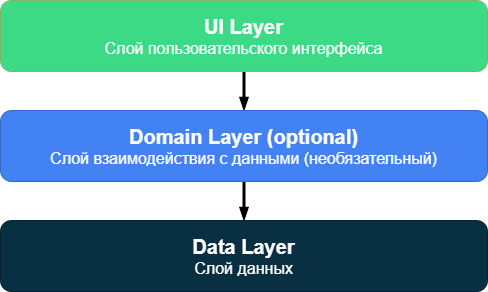
\includegraphics[width=\textwidth]{flesh/arch/uil-dol-dal.png}
	\caption{\label{fig:arch_uil_dol_dal}Схема архитектуры MVP}
\end{figure}

\subsection*{Обзор слоёв:}
\begin{description}
	\item[Слой пользовательского интерфейса] Этот слой иначе называют презентационным слоем. Его назначение – отображать данные приложения в том или ином виде на экране устройства. При изменении данных, взаимодействии с пользователем или поступлении внешнего ввода интерфейс должен соответствующим образом реагировать и отражать изменения.
	\item[Слой данных] Слой данных приложения содержит в себе «бизнес-логику». Бизнес-логика – это то, в чем есть суть приложения. Это правила, указывающие, как приложение создает, сохраняет и изменяет данные.
	Слой данных состоит из репозиториев, каждый из которых может содержать неотрицательное количество источников данных. Репозиторий создается на каждый отдельный тип данных, обрабатываемый в приложении.
	\item[Слой взаимодействия с данными] Иначе – слой доменов. Является опциональным слоем, расположен между презентационным слоем и слоем данных.
	Обычно представляет собой инкапсуляцию бизнес-логики, если она переиспользуется разными ViewModel объектами или если она достаточно объемная и сложная.
\end{description}

В минимально рабочем прототипе результирующего приложения также используется эта схема классической архитектуры.
Поскольку приложение работает с данными геолокации, в коде создан класс LocationEntity, отвечающий за единичную запись о геолокации устройства в конкретный момент времени. 
Он связан с объектами репозитория данных и доступа к данным. 
Эти объекты представляют собой слой данных в приложении.

Как такового слоя доменов в приложении нет, потому далее имеет смысл описать презентационный слой.

В приложении слой пользовательского интерфейса представлен следующими объектами:
\begin{description}
	\item[LocationUpdateViewModel] объект типа ViewModel, связывающий изменения в данных с изменениями в макете и его элементах;
	\item[LocationUpdateFragment] компонент типа Fragment, описывающий макет с отображаемым на экране содержимым и связанную с ним логику.
\end{description}

Таким образом с помощью применения стандартных компонентов и подходов к архитектуре реализуется корректный процесс работы с данными и интерфейсом в приложении под Android. 


\section{Компоненты бизнес-логики приложения}
\subsection{Сервисы}
Для управления ходом игры были созданы следующие сервисы:
\begin{description}
	\item[ScenarioService] Сервис, управляющий запуском и остановкой игровой сессии.
	\item[LocationService] Сервис, управляющий запуском и остановкой отслеживания геолокации в реальном времени.
	\item[HealthProtectionService] Сервис, обеспечивающий защиту здоровья игрока.
\end{description}
\smallskip
Дальше представлено более развёрнутое описание каждого из них.

\subsubsection*{ScenarioService}
Так как ScenarioService обеспечивает работу игровой сессии для него была включена настройка работы в фоне. Также этот сервис отвечает за запуск и остановку других игровых сервисов. 

ScenarioService не содержит в себе прямых методов запуска и остановки, которые можно было бы вызвать из активности, напротив, в нем используется встроенный механизм привязки сервисов Android: на событие привязки к активности и отвязки от активности происходит запуск с инициализацией и разрушение сервиса, соответственно.
\subsubsection*{LocationService}
Так как LocationService отвечает за бесперебойное получение данных о геолокации в реальном времени и должен уметь работать в фоне, он был реализован в виде стандартного сервиса Android. Так же как и ScenarioService, он не имеет методов для запуска и остановки, вызываемых из других компонент, при этом он запускается на присоединении к ScenarioService и имеет методы для включения или отключения работы в фоне.

\subsubsection*{HealthProtectionService}
Защита здоровья является важным компонентом с точки зрения заботы о пользователе. Представляет из себя подключаемый к ScenarioService сервис по аналогии с LocationService. 

При старте запускается таймер обратного отсчёта со следующими контрольными точками:
\begin{description}
	\item[За $N$ минут до истечения таймера] через голосовой интерфейс и вибрацию производится уведомление пользователя о необходимости завершить тренировку.
	\item[По истечении таймера] через голосовой интерфейс и вибрацию производится уведомление пользователя о принудительном завершении тренировки с фактическим её завершением.
\end{description}
\smallskip
При этом следует заметить, что таймер будет срабатывать при активности игровой сессии. При ручном$\backslash$аварийном (не инициированном пользователем или компонентом защиты здоровья) завершении игровой сессии таймер сбрасывается и не срабатывает до следующего запуска игровой сессии, когда он будет инициализирован заново.

\subsection{Менеджеры}
Менеджер \textemdash\space служебный класс, реализующий паттерн проектирования Singleton, так что во время работы приложения существует всегда только один объект этого класса, содержащий обрабатываемые данные.

Такие объекты нужны для хранения некоторого состояния приложения и данных игровой сессии.

В приложении были созданы следующие менеджеры:
\begin{description}
	\item[GeofencingManager] Менеджер обработки точек интереса и доступа к ним.
	\item[ActionsManager] Менеджер, управляющий событиями (генерация, финализация) и доступом к ним.
	\item[ObstaclesManager] Менеджер, управляющий препятствиями (генерация, финализация) и доступом к ним.
	\item[ScenarioManager] Менеджер обработки и управления запущенным сценарием геймификации.
	\item[SoundManager] Менеджер воспроизведения аудиконтента.
	\item[TTSManager] Менеджер воспроизведения звуковых нотификаций.
\end{description}
\smallskip
Далее представлено более подробное описание каждого из них.

\subsubsection*{GeofencingManager}
Объект данного класса хранит в себе активные во время игровой сессии точки интереса на карте и содержит методы управления ими:
\begin{description}
	\item[getActiveEntry] возвращает активную точку интереса, по которой ведется отслеживание в данный момент;
	\item[storeGeofence] добавляет точку интереса в очередь на ожидание;
	\item[processNext] финализирует активную точку интереса, помечает следующую в очереди как актуальную;
	\item[reset] очищает очередь точек интереса, сбрасывает активную, отключает отслеживание.
\end{description}

\subsubsection*{ActionsManager}
Объект данного класса хранит в себе активные во время игровой сессии таймеры и объекты сюжетных действий, а так же содержит методы управления ими:
\begin{description}
	\item[processEventAction] метод инициализации события, вызывается из ScenarioManager при предобработке сценария. 
	\item[scheduleAction] метод сохранения и запуска таймеров события, вызывается из processEventAction.
	\item[clear] очищает сохраненные данные по событиям и сбрасывает активные таймеры.
\end{description}

\subsubsection*{ObstaclesManager}
Объект данного класса хранит в себе на время игровой сессии виртуальные препятствия, а так же содержит методы управления ими:
\begin{description}
	\item[setCurrent] метод задания активного препятствия и запуска таймеров.
	\item[finalize] метод финализации препятствия.
	\item[clear] метод для очистки состояния препятствий.
\end{description}

\subsubsection*{SoundManager}
Объект данного класса одновременно хранит в себе активные во время игровой сессии точки интереса на карте и содержит методы управления ими:
\begin{description}
	\item[playTrack] метод для проигрывания музыкального трека из вложенных в приложение ресурсов.
	\item[stop] метод для остановки трека.
	\item[clear] метод для очистки состояния проигрывателя.
\end{description}

\subsubsection*{TTSManager}
Объект данного класса одновременно хранит в себе активные во время игровой сессии точки интереса на карте и содержит методы управления ими:
\begin{description}
	\item[speak] метод для озвучки голосовых инструкций системой TTS.
	\item[stop] метод для остановки озвучки голосовой инструкции через TTS.
\end{description}

\subsubsection*{ScenarioManager}
Объект данного класса так же, как и ScenarioService, является своего рода оркестратором описанных выше менеджеров. 
Содержит следующие методы:
\begin{description}
	\item[initialize] метод инициализации и предобработки сценария в заданном формате.
	\item[initializeCurrentChapter] метод инициализации текущей главы в рамках сценария.
	\item[runScenario] метод для запуска игровой сессии по загруженному сценарию.
	\item[finishChapter] метод завершения главы загруженного сценария по завершении игровой сессии.
	\item[clear] метод для очистки состояния менеджера.
\end{description}

\subsection{Получатели широковещательных сообщений}
\chapter{Геймификация бега}
Для геймификации бега была придумана концепция интерактивного сюжета, в рамках которой игрок оказывается в некой ситуации, разворачивающейся по мере прохождения точек интереса на карте. Также по мере развития сюжета игроку предлагаются некоторые препятствия, которые он должен физически обойти.
\section{Интерактивный сценарий}
Интерактивный сценарий представляет из себя иерархическую структуру данных cо вложенными объектами разного типа.
Техническая реализация сценария представляет из себя JSON-файл с жёстко заданной структурой. Основные компоненты сценария приведены на рис. \ref{fig:scenario_components}.

На схеме представлены следующие объекты:
\begin{description}
	\item[Chapter] Глава. Представляет из себя единицу геймифицированной тренировки, содержит собственный набор игровых объектов, актуальных для конкретной игровой сессии, как-то: Игровые события и Точки интереса на карте.
	\item[Event] Игровое событие. Игровые события описаны подробнее в разделе \ref{sec:events}.
	\item[Geofencing] Точки интереса на карте. Информация о точках интереса на карте представлена в разделе \ref{sec:geofencing}.
\end{description}

\begin{figure}[H]
	\centering
	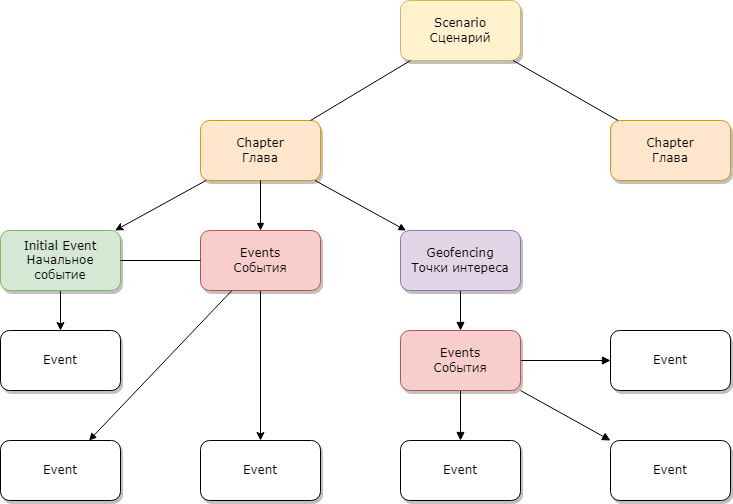
\includegraphics[width=\textwidth]{flesh/runGamification/scenario.png}
	\caption{\label{fig:scenario_components}Схема компонентов сценария}
\end{figure}

\section{Действия, производимые игрой}
\label{sec:actions}
Во время активной сессии игра может вызывать различные действия, основываясь на их контексте. Под контекстом будем понимать один из трёх над-родительских для действия объектов:
\begin{itemize}
	\item Начальное событие главы.
	\item Промежуточное событие главы.
	\item Событие для точки интереса на карте.
\end{itemize}
У каждого действия есть свой набор атрибутов, при этом у каждого действия обязательно есть следующие методы:
\begin{description}
	\item[initTimer] Данный метод возвращает инициализированный объект типа CountDownTimer, представляющий из себя таймер обратного отсчёта, по истечении которого будет запущен код, начинающий выполнение игрового действия. Такая реализация позволяет планировать действия на будущее в рамках активной игровой сессии.
	\item[finishTimer] Данный метод может не требоваться для действия, поэтому он возвращает  nullable объект типа CountDownTimer?, представляющий из себя таймер обратного отсчёта, по истечении которого будет запущен код, завершающий выполнение игрового действия. Такая реализация позволяет финализировать запущенные действия и валидировать результат их выполнения, если это необходимо.
\end{description}
\smallskip
Актуальная версия приложения имеет возможность вызывать два типа игровых действий:
\begin{itemize}
	\item Воспроизведение аудиоконтента.
	\item Генерация виртуального препятствия.
\end{itemize}
\smallskip
Далее рассмотрим их подробнее.

\subsection*{Действие воспроизведения аудиоконтента}
Данное действие воспроизводит заданный в файле сценария аудиотрек из вложенных в приложение ресурсов.

Этот вид действия не требует таймер финализации, т.к. для запуска трека достаточно только таймера запуска, и после его выполнения не требуется проводить проверки.

\subsection*{Действие генерации виртуального препятствия}
Данное действие генерирует заданное в файле сценария препятствие из реализованных в приложении. Детальная информация о виртуальных препятствиях представлена в разделе \ref{sec:obstacles}.

Это действие обязательно имеет оба таймера, так как у препятствия есть метод запуска и метод финализации, проверяющий было ли препятствие преодолено.
 
\section{Система игровых событий}
\label{sec:events}
Игровое событие представляет из себя набор игровых действий с соответствующими их типам атрибутами, которые игра может вызвать в некоторый момент времени на протяжении игровой сессии.

В приложении предусмотрено три типа игровых событий:
\begin{description}
	\item [Начальное событие] Если задано, вызывается всегда в начале соответствующей главы сценария
	\item [Событие, привязанное ко времени] Обязательно имеет атрибут с задержкой в секундах от начала главы, и вызывается в соответствующий момент времени.
	\item [Событие, не привязанное ко времени] Как и предыдущий тип, данное событие вызывается в определённый момент времени, но, в отличие от предыдущего, задержка не задаётся в сценарии, а рассчитывается в момент генерации как псевдослучайное число между двумя границами из кода приложения.
\end{description}


\section{Система виртуальных препятствий}
\label{sec:obstacles}
Виртуальное препятствие является концептом, которого не существует в реальном мире, но он генерируется игрой и заставляет игрока выполнить какое-либо действие, связанное с бегом. Сейчас мы различаем следующие виды препятствий:
\begin{description}
	\item[Дикие собаки] Данное препятствие имитирует бег за игроком диких собак, которые могут нанести ему вред : для преодоления препятствия необходимо ускориться за определённое время.
	\item[Сильный ветер] Данное препятствие имитирует сильный ветер, сносящий игрока. Для преодоления препятствия необходимо ``подыграть'' игре и снизить скорость за определённое время.
\end{description}
\smallskip
Данные препятствия выбраны исходя из концепции интервальных тренировок и режима бега, при котором человеку необходимо чередовать ускорение и замедление в рамках одной игровой сессии.

У каждого препятствия есть атрибут статуса, принимающий одно из следующих значений:
\begin{description}
	\item[UNKNOWN] Неизвестный статус. Присваевается препятствию в случае непредвиденных технических ошибок. При штатной работе приложения препятствия с таким статусом отсутствуют.
	\item[ONGOING] Активное препятствие. Приложение ожидает завршения таймера для валидации состояния преодоления.
	\item[FAILED] Не преодолённое препятствие. По завершении таймера приложение определило, что игрок не преодолел препятствие.
	\item[SUCCEEDED] Преодолённое препятствие. По завершении таймера приложение определило, что игрок смог преодолеть препятствие.
\end{description}
\smallskip
Далее рассмотрим некоторые детали работы с виртуальными препятствиями.
\subsection*{Генерация препятствия}
При генерации препятствия происходят следующие действия:
\begin{enumerate}
	\item Сохранение препятствия как активного в менеджере препятствий.
	\item Сохранение препятствия в репозиторий сгенерированных препятствий.
	\item Вызов инициализирующего метода препятствия.
	\item Запуск голосовой инструкции о типе препятствия и способе его преодоления.
\end{enumerate}

\subsection*{Валидация препятствия}
После срабатывания таймера финализации действия, отвечающего за финализацию препятствия вызывается соответствующий метод активного препятствия из менеджера препятствий и происходит следующее:
\begin{enumerate}
	\item Определение статуса преодоления препятствия.
	\item Обновление сущности в репозитории.
	\item Запуск голосовой инструкции о результате преодоления препятствия.
\end{enumerate}

\section{Система точек интереса}
\label{sec:geofencing}
Для геймификации и имитации продвижения по сюжетной линии сценария была реализована возможность менять игровой контекст по достижении очередной точки интереса на карте.

Точка интереса на карте представляет из себя объект с географическими координатами, рядом дополнительных атрибутов и набором игровых событий, каждое со своими атрибутами. При нахождении устройства пользователя в некоторой окрестности актуальной на момент игровой сессии точки игра может вызвать событие из набора событий данной точки.

Обработка точек интереса на карте производится методами Geofencing (см. разделы \ref{subsec:geodata} и \ref{subsubsec:geofencing_manager}).

Игровые события, вызываемые на входе пользователя в отслеживаемую зону, технически и идейно соответствуют уже рассмотренным в разделе \ref{sec:events}.

Отслеживание входа устройства игрока в заданную зону производится в рамках следующих ограничений:
\begin{itemize}
	\item Отслеживание ведётся только во время активной игровой сессии.
	\item Отслеживается нахождение пользователя только относительно одной актуальной в данный момент времени точки интереса (а таковая может быть только одна).
	\item Отслеживается только вход в заданную радиусом область. Технически есть возможность также отслеживать длительное нахождение в ней и выход из этой области, но в рамках данной работы эти события не отслеживаются.
\end{itemize}
\chapter{Описание реализации вспомогательного функционала}
\section{Получение требуемых разрешений от пользователя}
В соответствии с требованиями Google к безопасности пользовательских данных в рамках работы приложений в ОС Android для выполнения каких-либо действий или сбора каких-либо данных может потребоваться запросить на это разрешение у пользователя.

При этом, нельзя так просто взять и запросить разрешение. Перед этим его нужно объявить в файле AndroidManifest (см. Рис. \ref{fig:arch_uil_dol_dal}) который содержит некоторую метаинформацию о приложении, как-то:
\begin{enumerate}
	\item Название приложения.
	\item Список компонент (активности, сервисы, получатели сообщений, и т.д.).
	\item Название пакета с кодовой базой.
	\item Указание на первичную активность.
	\item Список разрешений, которые приложение будет запрашивать и задействовать.
\end{enumerate}
\dots и многое другое.
Так, в разрабатываемом приложении были указаны следующие разрешения:
\begin{enumerate}
	\item Для доступа к наиболее точной геолокации устройства:
	\begin{itemize}
		\item ACCESS\_FINE\_LOCATION
		\item ACCESS\_COARSE\_LOCATION
	\end{itemize}
	\item Для работы в фоне:
	\begin{itemize}
		\item ACCESS\_BACKGROUND\_LOCATION
		\item FOREGROUND\_SERVICE
	\end{itemize}
	\item Для определения физической активности пользователя устройства (на будущее):
	\begin{itemize}
		\item ACTIVITY\_RECOGNITION
	\end{itemize}
		\item Для уточнения геолокации и связи с сетевыми сервисами:
	\begin{itemize}
		\item ACCESS\_NETWORK\_STATE
		\item INTERNET
	\end{itemize}
\end{enumerate}
\smallskip
\begin{figure}[H]
	\centering
	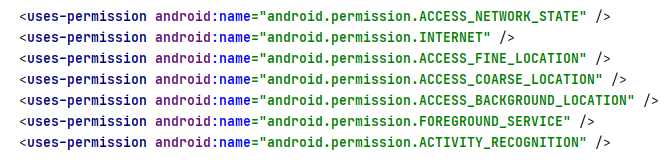
\includegraphics[width=\textwidth]{flesh/somefunc/manifest_permissions.png}
	\caption{\label{fig:manifest_permissions}Пример объявления разрешений в AndroidManifest.xml}
\end{figure}


После объявления разрешений требуется корректно их обработать в самом приложении – для каждого запрошенного разрешения проверить наличие разрешения от пользователя:
\begin{itemize}
	\item если разрешение есть \textendash\space продолжить выполнение инструкций приложения;
	\item если разрешения нет \textendash\space запросить его.
\end{itemize}
\smallskip


Проверку разрешений наиболее целесообразно производить в основной активности приложения. Однако, учитывая, что основная активность у нас сразу же инициализирует и отрисовывает фрагмент, отвечающий за отображение данных геолокации, было принято решение проверять разрешения в этом фрагменте.
Для проверки разрешения используется стандартный метод hasPermission контекста приложения (область методов и атрибутов приложения в конкретный момент времени, доступная в процессе выполнения приложения). 
В случае отсутствия разрешения инициализируется и отрисовывается один из фрагментов, содержащий макет с запросом на получение разрешения от пользователя. 

\section{Применение фрагментов}
Для замены фрагментов в содержимом, отображаемом на экране, используется встроенный объект supportFragmentManager~\autocite{android_fragment_manager}. Он позволяет в контексте атомарных транзакций управлять фрагментами. Алгоритм замены главного фрагмента фрагментом запроса разрешения выглядит следующим образом:
\begin{enumerate}
	\item Создать объект фрагмента, который следует отобразить на экране.
	\item Начать транзакцию.
	\item Передать инструкцию замены содержимого контейнера фрагмента созданным объектом.
	\item Сохранить операцию замены в конец стека операций транзакции.
	\item Применить транзакцию.
\end{enumerate}


\section{Организация хранения данных о геолокации устройства}
Как было описано в предыдущем разделе об архитектуре приложения, данные о геолокации хранятся в базе данных, доступ к которой производится через библиотеку Android Room, создающую некоторые абстракции для управления сущностями, объектами доступа к данным и объектами связи данных с макетом содержимого экрана.
Объект класса AppDatabase, наследующийся от системного RoomDatabase, реализует паттерн проектирования Singleton~\autocite{singleton}, доступен в единственном экземпляре на протяжении всей работы приложения и используется для следующих целей:
\begin{enumerate}
	\item Инициализация базы данных с нуля согласно автоматически сгенерированной схеме на основе известных приложению объектов типа Сущность.
	\item Инициализация репозитория с существующими данными, также реализующего паттерн проектирования Singleton, что делает его доступным в единственном экземпляре на протяжении всей работы приложения.
\end{enumerate}

\smallskip

\begin{figure}
	\centering
	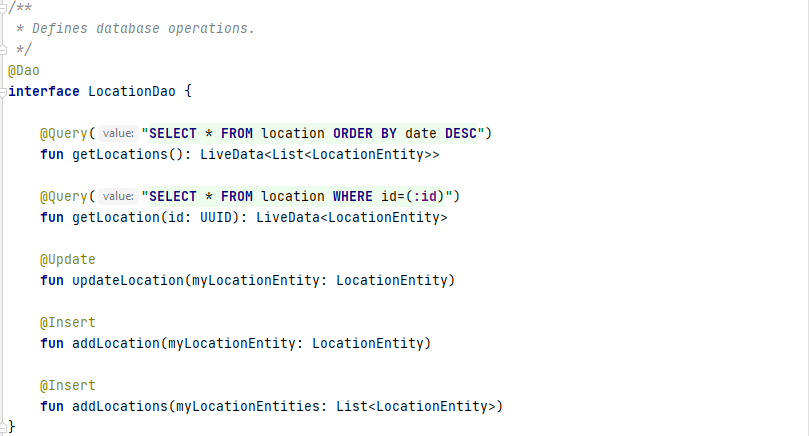
\includegraphics[width=\textwidth]{flesh/somefunc/location_dao.png}
	\caption{\label{fig:location_dao}Объявление методов объекта доступа к сохраненным данным геолокации}
\end{figure}

После инициализации базы и репозитория вся работа с данными производится с помощью методов объекта класса LocationDao (приведен на Рис. \ref{fig:location_dao}), который реализует CRUD модель доступа к содержимому репозитория.

\section{Получение данных о текущей геолокации устройства}
С помощью объекта LocationUpdatesBroadcastReceiver приложение подписывается на получение обновлений от сервиса геолокации Google Services – FusedLocationProviderClient.
Далее создается PendingIntent – ожидающее действие, которое при получении нового широковещательного сообщения с данными о геолокации запускает метод сохранения полученных данных в базу.
Доступ к сервису геолокации FusedLocationProviderClient производится через класс-обертку LocationManager, который отвечает за хранение флага активности отслеживания и настроек отслеживания, таких как частота отслеживания, приоритет получения данных и требуемая точность данных.

\section{Фоновое получение данных о геолокации}
В приложениях для ОС Android, как было описано ранее, используется концепция функциональных единиц – Activity (активностей). При этом в приложении всегда есть основная активность, которая запускается при открытии приложения. В ней инициализируют значения, запускают фоновые сервисы и указывают инструкции для отрисовки первичного содержимого экрана.
По умолчанию такая активность имеет название MainActivity. В ней мы создаем Intent («намерение» с некоторым действием), который запускает наш LocationService. 
При инициализации сервиса создается постоянное уведомление в шторку о работе приложения в фоне, в зависимости от версии ОС Android это делается по-разному.
Далее происходит запуск сервиса, в котором вызывается метод запуска отслеживания изменений геолокации из LocationRepository. Сервисы работают в фоне, поэтому им не требуется какое-либо представление в презентационном слое архитектуры приложения, при этом они могут обращаться к слою данных, что здесь и происходит.

\section{Связь данных с макетом содержимого экрана}
Именно за связь уже сохраненных данных о геолокации из базы и пользовательского интерфейса отвечает объект типа ViewModel – LocationUpdateViewModel: он содержит в себе вызовы соответствующих методов репозитория данных и больше ничего не делает.
Кроме того, для связи данных с макетом используются два механизма привязки объектов на этапе сборки:
\begin{description}
	\item[viewBinding] механизм привязки объектов макета к классу, содержащему инструкции по встраиванию макета в пользовательский интерфейс. Этот механизм позволяет не использовать устаревшую и неподдерживаемую конструкцию поиска объекта макета по его идентификатору – вместо этого после сборки проекта все элементы соответствующего макета доступны из автоматически генерируемого класса доступа к ним.
	\item[dataBinding] механизм действия, обратного viewBinding, позволяющий после сборки проекта использовать в макете содержимого пользовательского интерфейса содержимое объектов типа ViewModel.
\end{description}
\smallskip
Оба механизма включаются установкой соответствующих пакетов и заданием одноименных флагов в блоке buildFeatures конфигурационного файла системы сборки проекта Gradle – build.gradle (:app).


\section{Управление флагом активности отслеживания геолокации}
На основе LocationUpdateViewModel работает управление флагом состояния отслеживания: при нажатии на соответствующую кнопку в макете пользовательского интерфейса (включение/отключение отслеживания) производятся следующие действия:
\begin{enumerate}
	\item Запускается или останавливается сервис отслеживания.
	\item Вызываются методы LocationUpdateViewModel, запускающие или останавливающие отслеживание через отмену или активацию подписки на события изменения геолокации в LocationManager.
\end{enumerate}
 
\chapter{Оптимизация использования ресурсов устройства}
Приложение, работающее в фоне и производящее постоянные запросы определенно имеет большой потенциал для оптимизации по использованию ресурсов устройства. Далее приведены некоторые рассуждения относительно влияния постоянной работы приложения на состояние устройства и возможные варианты доработок приложения для улучшения пользовательского опыта и снижения нагрузки на устройство.

\section{Влияние частоты измерения геолокации на расход заряда аккумулятора устройства}
\subsection*{Аспекты, влияющие на расход заряда аккумулятора}
В первую очередь следует определить три аспекта~\autocite{battery}, с которыми напрямую связан повышенный расход заряда аккумулятора устройства:
\begin{description}
	\item[Точность определения геолокации] В общем случае – чем выше точность, тем больше потребление заряда.
	\item[Частота запросов данных датчиков геолокации] Чем чаще происходит опрос датчиков и их сообщение с источниками данных (спутники, сетевые устройства, сотовые вышки, и т.д.), тем выше расход заряда.
	\item[Время ожидания отклика сервиса геолокации] Меньшая скорость обычно требует меньше ресурсов аккумулятора.
\end{description}

\subsubsection*{Точность определения геолокации}
Этим параметром можно управлять с помощью специального метода setPriority, который принимает в качестве аргумента следующие значения:
\begin{description}
	\item[PRIORITY\_HIGH\_ACCURACY] в этом режиме приложение будет получать наиболее точные данные о геолокации устройства на основе всех возможных источников: GPS, WiFi, вышки сотовой связи и множество доступных на устройстве датчиков.
	\item[PRIORITY\_BALANCED\_POWER\_ACCURACY] этот режим представляет приложению достаточно точные данные о геолокации устройства, в щадящем для аккумулятора режиме: обращения к GPS производятся максимально редко, обычно используется комбинация запросов к WiFi и вышкам сотовой связи.
	\item[PRIORITY\_LOW\_POWER] данное значение точности задает более строгий режим экономии электроэнергии устройства: сервис геолокации опирается исключительно на данные вышек сотовой связи, не используя никакие другие источники. Такой подход дает грубое приближение к реальной геолокации устройства с точностью до части населенного пункта, при этом затрачивая минимум заряда аккумулятора.
	\item[PRIORITY\_NO\_POWER] в этом режиме данные геолокации переиспользуются из результатов запросов геолокации другими приложениями, для которых они уже были получены.
\end{description}


\subsubsection*{Частота запросов данных геолокации}
Этим параметром можно управлять с помощью следующих методов:
\begin{description}
	\item[setInterval] задает интервал за который геолокация будет запрашиваться конкретно для этого приложения;
	\item[setFastestInterval] задает интервал за который геолокация будет доставляться этому приложению с результатам запросов другими приложениями.
\end{description}
\smallskip
Хорошей практикой является указание максимально возможного значения первым методом, особенно для сбора геолокации в фоновом режиме.


\subsubsection*{Время ожидания отклика сервиса геолокации}
Значение этого атрибута задается с помощью метода setMaxWaitTime и, как правило, в несколько раз больше, чем значение, указанное в setInterval.
Этот атрибут откладывает доставку результатов определения геолокации, в таком случае за один раз может быть доставлен батч из нескольких результатов с изменениями геолокации.


\subsection*{Способы экономии заряда}
Учитывая специфику приложения, можно отметить следующие факторы, важные для определения стратегии определения методов оптимизации:
\begin{itemize}
	\item Крайне нежелательно откладывать доставку результатов с данными геолокации, так как данные нужны в режиме реального времени.
	\item Физическая активность в открытом пространстве с элементами геймификации может быть потенциально травмоопасной и для минимизации рисков взаимодействия с объектами окружающей инфраструктуры, действительно несущими риск нанесения травм пользователю, требуется знать наиболее точное местоположение пользователя с его устройством.
\end{itemize}
\smallskip
Исходя из всего вышеперечисленного можно предпринять следующие попытки по оптимизации расхода заряда устройства:
\begin{enumerate}
	\item Установить точность на уровне не ниже PRIORITY\_BALANCED\_POWER\_ACCURACY.
	\item Установить частоту запросов к сервисам геолокации не ниже раза в 20 секунд.
	\item Установить время ожидания доставки обновлений не менее 5 секунд.
\end{enumerate}
\smallskip
Эти значения предположительно принесут оптимизацию расхода батареи работой приложения примерно в 3 раза (учитывая текущие значения в минимально рабочем прототипе приложения).


\section{Влияние работы приложения на используемую память устройства}
На основе схемы базы имеется приблизительный~\autocite{sqlite_datatypes} объем данных в одной строке, представляющей собой один объект класса LocationEntity – 90 байт. При получении до 100 объектов в секунду приложение производит 900 байтов. Так приложение займет объем в 1 Гб за примерно 300 часов непрерывной работы. Совершенно очевидно, что такой объем данных, создаваемых и хранимых приложением, не нужен ни приложению, ни пользователю устройства. 
В качестве возможности избежать такой нерациональной траты памяти предлагается:
\begin{enumerate}
	\item Предусмотреть процессы периодической очистки сохранённых данных, возможно, оставляя данные за последние $N$ часов, где $N$ строго меньше $150$.
	\item Рассмотреть возможность сохранять не все пришедшие в батче данные об изменениях локации, а только часть в $M/K$, где $K$ \textemdash\space количество изменений, пришедших в батче, а $M$ \textemdash\space количество записываемых из них изменений такое, что $1 \le M \le [K/2]$.
\end{enumerate}
\smallskip
Такие меры сохранения памяти устройства определённо повысят качество пользовательского опыта и снизят влияние от использования разрабатываемого приложения на другие приложения потенциального пользователя и его устройство в целом.
 
\chapter{Программная реализация сбора биометрии}
В качестве дополнительного метода защиты здоровья пользователя было принято решение анализировать его пульс во время тренировок.
Получение пульса возможно путём взаимодействия с устройствами сбора пользовательской биометрии, такими как умные часы и браслеты.

\section{Выбор метода сбора биометрии}
Для определения доступных возможностей был проведён сравнительный анализ нескольких методов получение биометрических данных:
\begin{itemize}
	\item Выполнение запросов к датчикам биометрии напрямую на носимом устройстве.
	\item Выполнение запроса к сервисам биометрии Google.
	\item Выполнение запроса к агрегатору биометрии на устройстве от Google.
	\item Выполнение запроса к агрегатору биометрии вендора носимых устройств.
\end{itemize}
\smallskip
Результат сравнительного анализа представлен в таблице \ref{tab:biometrics_comparison}.

\newcolumntype{s}{>{\hsize=.4\hsize}X}
\newcolumntype{t}{>{\hsize=.25\hsize}X}

%table
\begin{table}[H]
	\centering
	\caption{\label{tab:biometrics_comparison}Результаты сравнительного анализа методов получения биометрии}
	\small
	\begin{threeparttable}
		\begin{tabularx}{\textwidth}{sXt}
			\toprule
			Метод сбора \newline биометрии
			& Описание и ограничения
			& Вывод \\
			\midrule\midrule
			Прямой запрос к датчикам носимого устройства
			& Предоставляет полные\tnote{1} данные в реальном времени\tnote{2}. \newline Для доступа к датчикам носимого устройства требуется сборка приложения-компаньона для загрузки на носимое устройство
			& Не\newline подходит \\\midrule
			Запрос к сервисам биометрии Google
			& Предоставляет полные исторические\tnote{3} данные. \newline Для доступа к биометрии требуется платный аккаунт, с которого отправляются запросы к API Google, подразумевается постоянное наличие соединения с Интернетом.
			& Не\newline подходит \\\midrule
			Запрос к агрегатору биометрии на устройстве от Google
			& Предоставляет полные\tnote{1} исторические\tnote{3} данные. \newline Реализуется через запущенный в тестирование в 2022 г. проект Google Health SDK. Требуется установка приложения-компаньона на устройство, настройка синхронизации и предоставление разрешений пользователем. Представляется неинтуитивным и требует много дополнительных действий со стороны конечного пользователя.
			& Не\newline подходит \\\midrule
			Запрос к агрегатору биометрии вендора носимых устройств
			& Предоставляет полные\tnote{1} исторические\tnote{3} данные. \newline Для доступа к данным требуется подключение к приложению пакета SDK соответствующего вендора.
			& Подходит \\
			\bottomrule
		\end{tabularx}
		\smallskip
		\footnotesize
		\begin{tablenotes}
			\item[1] Без ограничений на объем получаемых данных и с обширным списком доступных биометрических показателей.
			\item[2] Предоставляется возможность отслеживать изменения значений показателя в реальном времени и реагировать на них.
			\item[3] Предоставляется возможность выгрузить историю значений показателя за некоторый временной интервал в прошлом.
		\end{tablenotes}
	\end{threeparttable}
\end{table}
\smallskip

Исходя из результатов сравнительного анализа методов получения биометрических данных, было принято решение использовать запросы к агрегатору данных конкретного вендора носимых устройств.
С учетом особенностей получения вендорских данных концепция второй системы защиты здоровья игрока через отслеживание пульса была изменена в пользу отслеживания истории изменения пульса на протяжении тренировки в момент её завершения.

\section{Определение вендора биометрических данных}
Сейчас на рынке присутствует большое количество различных производителей умных носимых устройств:
\begin{multicols}{2}
\begin{itemize}
	\item Xiaomi;
	\item Huawei;
	\item Garmin;
	\item Samsung;
	\item Apple;
	\item Honor.
\end{itemize}
\end{multicols}

и многие другие.


В рамках данной работы требовалось собрать минимальный рабочий прототип приложения для геймификации бега, поэтому интеграция со всеми вендорами представляется избыточной и, в некотором роде невозможной. 

С учётом приведённого выше аргумента и наличия в прямой доступности экземпляра умных часов Samsung было принято решение интегрироваться с Samsung Health SDK. 

В следующем разделе опишем некоторые подробности интеграции с выбранным вендором.

\section{Особенности реализации сбора биометрии через Samsung Health SDK}
Для интеграции с Samsung Health SDK~\autocite{shsdk_intro} требуется произвести ряд шагов:
\begin{enumerate}
	\item Принять условия пользовательского соглашения на сайте Samsung.
	\item Скачать в каталог проекта приложения на Android собранную библиотеку SDK в формате JAR.
	\item Подключить ее в систему сборки gradle.
\end{enumerate}
\smallskip
После этого можно приступать к получению и обработке биометрических данных от Samsung.

\subsection{Получение данных}
Samsung Health SDK позволяет получать широкий набор биометрических данных:
\begin{multicols}{2}
	\begin{itemize}
		\item Пройденные шаги;
		\item Пройденные этажи;
		\item Длительность сна;
		\item Фазы сна;
		\item Статистика питания;
		\item Объем выпитой воды;
		\item Объем принятого кофеина;
		\item Артериальное давление;
		\item Частота сердечных сокращений;
		\item Антропометрические показатели:
		\begin{itemize}
			\item Рост;
			\item Вес;
			\item Температура тела.
		\end{itemize}
		\item Мышечная масса;
		\item Некоторые биохимические показатели крови.
	\end{itemize}
\end{multicols}
\smallskip
Часть показателей собирается системами вендора в автоматическом режиме (например, шаги, пульс, длительность сна), тогда как другие \textemdash\space вносятся пользователем самостоятельно в вендорское приложение-компаньон.

В рамках данной работы требуется получить пульс пользователя~\autocite{shsdk_heart_rate}. Этот показатель рассчитывается автоматически на основе данных с умных часов Samsung, подключённых к телефону пользователя.

Здесь стоит ещё раз отметить особенность работы с Sasmsung Health SDK: данный подход не позволяет получать информацию в реальном времени. Дальнейшее исследование показало, что на от часов к устройству данные передаются с большой задержкой и получение псевдо-онлайн данных также не возможно.

\subsection{Особенности работы с Samsung Health SDK}
Для работы с вендорским агрегатором данных Sasmsung Health SDK требуется получить специальный партнерский код доступа~\autocite{shsdk_dev_mode} на портале Samsung Developers. Код привязывается к названию пакета Android приложения, использующего данные биометрии вендора.

После этого алгоритм запроса биометрических данных выглядит следующим образом:
\begin{enumerate}
	\item Запросить у пользователя разрешения да его биометрические данные.
	\item Создать объект класса HealthDataRepository~\autocite{shsdk_data_store}.
	\item Выполнить запрос подключенному репозиторию с указанием требуемых типов биометрических данных.
\end{enumerate}
\smallskip
Пример работы с Samsung Health SDK приведен в приложении \ref{list_sec:shm}.
\chapter{Анализ результатов тестирования приложения}


\pagebreak

\Conc
В рамках данной работы было сделано следующее:
\begin{enumerate}
	\item Разработана схема геймификации занятий бегом и ходьбой на основе интервальных тренировок, имитация которых представлена в виде виртуальных препятствий.
	\item Спроектировано и собрано мобильное приложение под ОС Android.
	\item Реализована работа с продвинутым сервисом обработки геоданных.
	\item Настроена система базовой защиты здоровья пользователя, в виде ограничения длительности тренировки.
	\item Разработан формат задания интерактивных геймифицирующих занятие сценариев, через которые можно задавать безопасный беговой маршрут с точками интереса на карте.
	\item Расписаны два тестовых сценария геймификации, вшитых в приложение, с загруженным аудиосопровождением.
	\item Успешно проведено как автоматическое, так и закрытое пользовательское тестирование разработанного приложения.
\end{enumerate} 
\smallskip

Исходный код разработанного приложения и актуальная собранная версия доступны по ссылке: \url{https://github.com/AlKempl/RunListenRun}.


Исходный код данной выпускной квалификационной работы и актуальная собранная версия доступны по ссылке: \url{https://github.com/AlKempl/mmcs_master_thesis}.




\pagebreak

%https://www.zotero.org/alkempl/items/BMGR99L5/library -- source
%\nocite{*} -- print all not cited items from bibliography
\printbibliography[
heading=bibintoc,
title=Список литературы
]

\pagebreak

\appendix

\ifthenelse{\value{worktype} > 1}{%
	\addtocontents{toc}{%
		\protect\renewcommand{\protect\cftchappresnum}{\appendixname\space}%
		\protect\addtolength{\protect\cftchapnumwidth}{\widthof{\appendixname\space{}}  - \widthof{Глава }}%
	}%
}{
	\addtocontents{toc}{%
		\protect\renewcommand{\protect\cftsecpresnum}{\appendixname\space}%
		\protect\addtolength{\protect\cftsecnumwidth}{\widthof{\appendixname\space{}}}%
	}%
}

\addtocontents{toc}{\protect\setcounter{tocdepth}{1}}

идфридфр

\end{document}
